\section{Introduction}
\label{sec:intoduction}
The emergence of distributed and parallel systems in the technical landscape has improved fault tolerance, efficiency, and dependability of systems, as well as tackling the issues of scalability, performance, and more \cite{b1}. One such implementation of distributed and parallel systems in the domain of mobility and logistics is truck platooning. Truck platooning is a driving technique in which a convoy of trucks travels close to one another while being linked by advanced driver assistance systems and wireless technologies as visualized in Figure \ref{img:truckplatooning}. The convoy's lead truck, which is equipped with sensors and communication systems, sets the pace and directs its progress, while the following trucks imitate its actions, including braking and acceleration. This helps with traffic flow optimization, enhances road safety, increases fuel efficiency and cost savings, and reduces environmental impact \cite{b2}. 
\begin{figure}[ht]
    \centering
    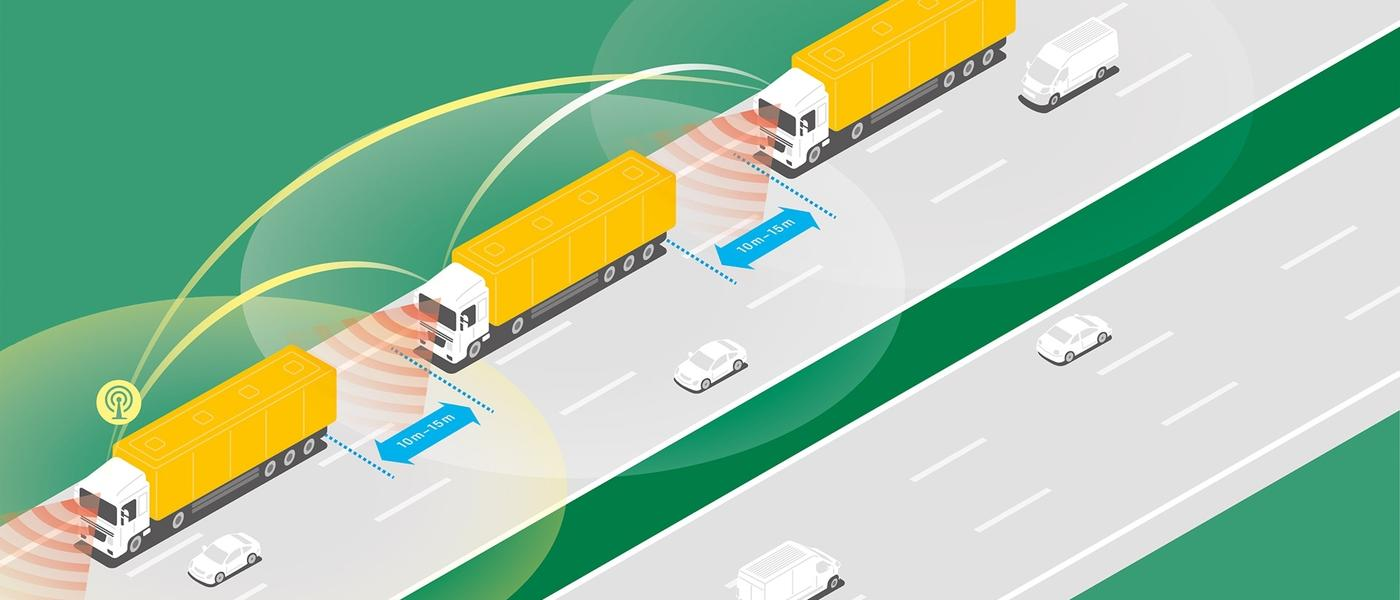
\includegraphics[width=0.5\textwidth]{images/truckplatooning.jpg}
    \caption{Truck Platooning \cite{b3}}
    \label{img:truckplatooning}
\end{figure}